\chapter{Introductions to QuickCheck}
\label{APP:QUICKCHECK}
\lstset{style=erlang}
\label{SEC:QuickCheckIntro}
Lets say that one created a \emph{sort} function that takes a list $Xs$ of any
sortable items and returns the sorted version $Ys$ of $Xs$. Then one can specify
certain properties that must hold for to the sort function. For instance:

\noindent The arity of $Y$ must be the same.
\begin{equation}
        |Xs| = |Ys|
\end{equation}

\noindent The elements of $Ys$ must actually be sorted.
\begin{equation}
    y_{i-1} \leq y_i, \forall y_i \in Ys, i \neq 0
\end{equation}

\noindent For all permutations $Pe(Xs)$ holds:
\begin{equation}
sort(Zs) = Ys, \forall Zs \in Pe(Xs)
\end{equation}

\noindent The sets $Xs$ and $Ys$ contains the same elements.
\begin{equation}
        x \in Xs \leftrightarrow x \in Ys
\end{equation}
Instead of specifying own test cases QuickCheck makes it possible to write such
properties, automatically generates test cases and checks that the properties
specified actually holds.

When testing C code with QuickCheck one uses state based testing. Which means
that a model state $S$ is passed around and checked against API calls according to
figure \ref{FIG:API_CALLS}.

\begin{figure}[!h]
  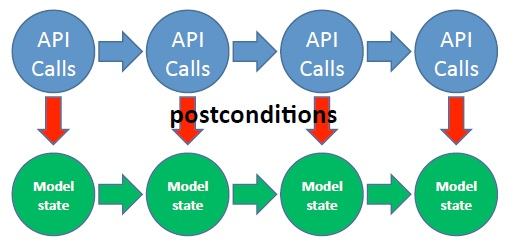
\includegraphics{pictures/api_calls.jpg}
  \caption{Shows state based testing against API and model state}
  \label{FIG:API_CALLS}
\end{figure}

A property in QuickCheck is written in the following way.
\lstset{style=erlang}
\begin{lstlisting}
prop() ->
  ?FORALL(Cmds, commands(),
          begin
            ... = run_commands(Cmds)
          end).

command(S) ->
      [{call, Mod, CFunction, arg_generator(S)},
        ... ].
\end{lstlisting}

The function \emph{commands()} is a generator and looks in the module after a
function called \emph{command(S)} which takes a state and returns a list of
functions that one want to test.

Every command has, additional to the command definition,
a precondition, postcondition and a next state function. For more information
about this, see section \ref{SEC:EQC_STATEM}.

After the property has been implemented, it can be tested by:

\begin{lstlisting}
eqc:quickcheck(prop()).
\end{lstlisting}

One can define how many tests QuickCheck should execute and also if the
states of the model should be shown:

\begin{lstlisting}
eqc:quickcheck(eqc:numtests(N, eqc_statem:show_states(prop()))).
\end{lstlisting}

\section{QuickCheck Modules}
The commercial version QuickCheck consist of several Erlang modules.
%%eqc
\subsection{eqc}
The module \emph{eqc} is the main QuickCheck module. This module defines a lot
of macros that can be used when writing properties and also basic functions
like \emph{quickcheck}.

\subsection{eqc\_gen} The module is used for generation of test cases. The module
contains various functions and macros for this purpose. There are some
predefined generators, for instance for integers and characters etcetera, but it
is quite easy to construct a generator for almost any data type. Just to get the
idea follows code for a string generator.
\begin{lstlisting}
    ?LET(Pat, nat(), vector(Pat, char()))
\end{lstlisting}
The macro \emph{?LET} binds a generated value from the second argument, to \emph{Pat} which can be
used in the third argument. The above code binds a natural number, from the
generator \emph{nat()}, to \emph{Pat} and creates a vector with length
\emph{Pat} of characters.

A generator can also be weighted, or in other words certain values can be more
likely to be generated then others.

\begin{lstlisting}
?LET(Pat, nat(), vector(Pat,
                        frequency([{1, choose(0,127)},
                                   {3, 32}])))
\end{lstlisting}
The code above will also generate a string of length \emph{Pat}, but the
generation of the white space character will be 3 times more likely to happen
than then a uniformly random character.

%%% eqc_c
\subsection{eqc\_c} Contains the C-testing interface. In other words how to
communicate with C-code.

\begin{lstlisting}
eqc_c:start(suit, [{c_src, "suit_api.h"},
                   {additional_files, ["myprog.o"]}])
\end{lstlisting}
The code above starts the C-program \emph{myprog.o}, and an Erlang module is
created with the name of the first parameter, \emph{suit}. This module can now
be used within Erlang to get information about the C-program. For example the
following function, that counts the number of spaces in a string, might be
declared in \emph{suit\_api.h} and defined in the \emph{myprog.o}.
\lstset{style=c}
\begin{lstlisting}
extern int spaces(char *str)
\end{lstlisting}
Then we can make the following call in the Erlang:
\lstset{style=erlang}
\begin{lstlisting}
suit:spaces("this is a string")
\end{lstlisting}
If the function \emph{spaces} is defined correctly the output will be 3.
%%% eqc_statem
\subsection{eqc\_statem}
\label{SEC:EQC_STATEM}
Offers state based testing. A command has a definition, precondition,
postcondition, and a next function. If we wanted to test \emph{spaces} function
one may write:
\begin{lstlisting}

% Defines the initial model state
initial_state() ->
  [].

% Takes the model state as a parameter
% Returns a tuple of the format
%   {call,Module,Function_to_call,Arguments_to_function}
spaces_command(_State) ->
  % Generates a natural number, binds it to Pat and generates a
  % list with length Pat with elements of type char
  Xs = ?LET(Pat,nat(),vector(Pat,char())),
  {call,?MODULE,spaces,[Xs]}.

% The actual call to the C-code
spaces(Xs) ->
  suite:spaces(eqc_c:create_string(Xs)).

%Takes the model state as a parameter
%The spaces function has no preconditions
spaces_pre(_State) ->
  true.

%Pramaters: S = ModelState, Args = arguments to the command
%Defines what should hold after the command
spaces_post(_S,Args=[Arg],Ret) ->
  length(lists:filter(fun(X) -> X == 32 end,Arg)) == Ret.

%Parameters: S    = model sate before the call,
%            Ret  = return value from command,
%            Args = argements to command
%Return the new model sate after the command is called
spaces_next(S,_Ret,_Args) ->
  S.
\end{lstlisting}

Noticeable is that only the post function may depend on the C-code. QuickCheck
has a generation step where tests are generated according to the precondition
and the model state. The C-code is run first after the generation step and can
only be used to check postconditions. This is actually what one want because it
would be pointless to execute a program and then test it depending on the
execution of the same program and not the model itself. For instance if we let
the next state function depend on the C-program, then the model will be
faulty
if the C-program has incorrect behaviour.

\begin{comment}
==============================================================================
  N�r exemplet ovan �ndras, skriv om detta stycke ocks�.
==============================================================================
\end{comment}
The example above is actually not state dependent since \emph{spaces} only
depend on the argument string. However one can imagine the same function being
dependent on some global variable and according to that variable change its output.
%car_xml
\subsection{car\_xml}
Additional to the commercial version, there is a \emph{car} module. This module is
specifically created to parse AUTOSAR XML configuration files.

%% relevans?
\subsection{Other modules}
\label{APP:SEC:OTHERMODULES}
There are also other modules; for instance a module for mocking C-code. Or in
other words, if one has a C-function that is declared but the
definition is missing, one can simulate its output. This is
however not used in this thesis.

%%%%%%%%%%%%%%%%%%%%%%%%%%%%%%%%%%%%%%%%%%%%%%%%%%%%%%%%%%%%%%%%%%%%%%%%%%%%%%%%


\chapter{The Watchdog Manager (WdgM)}
The watchdog is a basic AUTOSAR module. It's purpose is to supervise a programs
execution by triggering hardware watchdogs entities. For the hole description of
the module see the AUTOSAR specification.

\section{Supervision, Checkpoints and Graphs}
The watchdog supervises the execution of so called \emph{Supervised Entities}.
Important places in a supervised entity are marked as checkpoints. There are at
least one checkpoint for every supervised entity. The checkpoints and
transitions between checkpoints are defined as graphs. Checkpoints and
transitions between checkpoints within a given supervised entity are marked as
internal graphs. There may however be transitions between checkpoints of
different supervised entities, such graphs are marked as external graphs.
Available graphs are supplied by the configuration. There may be different
graphs for different modes of the watchdog manager.
%Lite matematiska utryck kanske?

There are three supervision algorithms to verify the correctness of supervised
entities.
\begin{itemize}
\item Logical Supervision: \\
Logical supervision verifies if graphs are executed in the correct order. \\ Let
$G = (V,E)$ be a internal graph for a supervised entity $S$ such that $\forall c_k
\in V \rightarrow c_i \in S$. For the graph $G$ there exist a start checkpoint
$c_s \in V$ and a final checkpoint $c_f \in V$. The logical supervision
checks that the first checkpoint $c_1$ that is reached has the property $c_1 =
c_s$ and for every reached checkpoint $c_j$ there exists an edge
$(c_{j-1},c_{j}) \in E, j \neq 1$.
\item Alive Supervision: \\
  Alive supervision periodically verifies the timing of transitions and
checkpoints reached in a graph.
\item Deadline Supervision: \\
  Deadline supervision does the same as alive supervision but aperiodically.
\end{itemize}

\section{Global Status}
The global status represents the current state of the whole watchdog
manager. There are five different statuses.
\begin{itemize}
\item WDGM\_GLOBAL\_STATUS\_DEACTIVATED \\
  The watchdog manager is in a resting state, deactivated, and will not execute
  any supervision functions.
\item WDGM\_GLOBAL\_STATUS\_OK \\
  The watchdog manager is in a correct state.
\item WDGM\_GLOBAL\_STATUS\_FAILED \\
  A failure has occurred for an alive supervision and the watchdog is configured
  to have a tolerance against this kind of error.
\item WDGM\_GLOBAL\_STATUS\_EXPIRED \\
  A fault has happened and the watchdog is configured to postpone the error
  reaction. In contradiction to
  \emph{WDGM\_GLOBAL\_STATUS\_FAILED} there is no recovery mechanism for this
  state and the watchdog manager will eventually reach the state
  \emph{WDGM\_GLOBAL\_STATUS\_STOPPED}.
\item WDGM\_GLOBAL\_STATUS\_STOPPED \\
  This is an absorbing state of the watchdog state machine. Recovery mechanisms
  will be started and usually a watchdog reset will occur.
\end{itemize}
The different statuses are related to each other according to figure~\ref{APP:FIG:GLOBALSTATUS}.
There is only a small number of functions that is allowed to change the global
status; those are the main function, the initialization function and the
de-initialization function. The main function decide the next global status by
checking the local statuses of the supervised entities and the current global
status. The initialization function should only be able to change the global
status from deactivated to ok, and the de-initialization function from ok to deactivated.

\begin{figure}[!ht]
  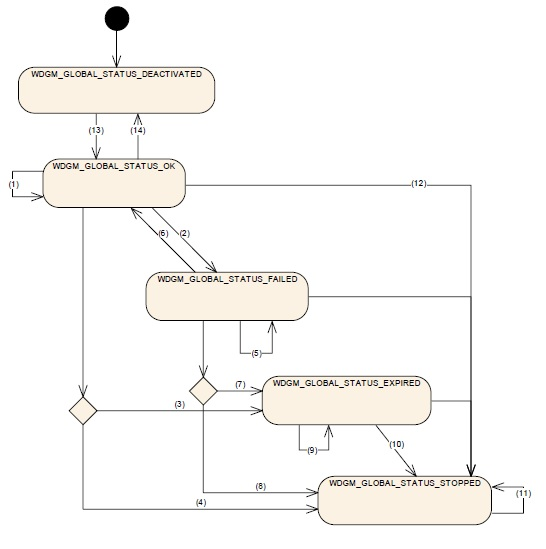
\includegraphics{pictures/globalstatuses}
  \label{APP:FIG:GLOBALSTATUS}
  \caption{The possible global statuses represented as a graph}
\end{figure}

\section{Local Status}
A local status is a status of one supervised entity and could be set according
to the current local status and the results of the supervision functions. There
are four different local statuses. Init setmode mainfunction

\begin{itemize}
  \item WDGM\_LOCAL\_STATUS\_DEACTIVATED\\
    If a supervised entity is set to deactivated, it will not be checked by the
    supervision functions.
  \item WDGM\_LOCAL\_STATUS\_OK\\
    The supervised entity is in a correct state.
  \item WDGM\_LOCAL\_STATUS\_FAILED\\
    Alive supervision for the supervised function has failed.
  \item WDGM\_LOCAL\_STATUS\_EXPIRED\\
    A fault has been observed within the supervised function. The main function
    will save the identification of the first supervised entity which reach this
    state.
\end{itemize}
Figure \ref{APP:FIG:LOCALSTATUSES} describes the state machine for the local
status of a supervised entity.

\begin{figure}[!ht]
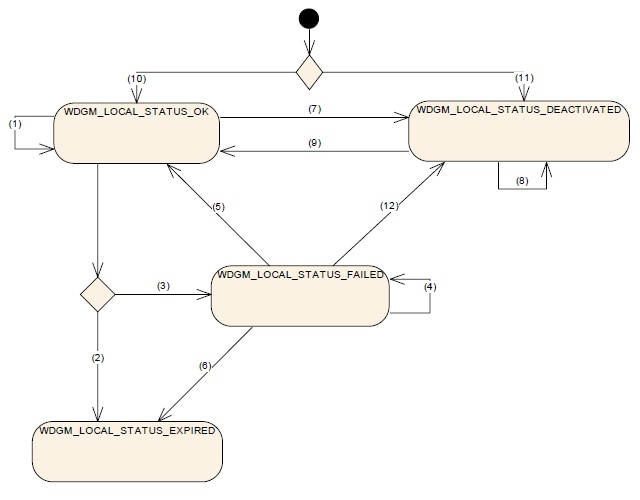
\includegraphics{pictures/localstatuses}
\label{APP:FIG:LOCALSTATUSES}
\caption{The possible local statuses represented as a graph}
\end{figure}

\section{API functions}
\label{APP:API_CALLS}
\subsection{WdgM\_Init}
Initializes the watchdog manager by setting, among other things, the local
status of all supervised entities to either WDGM\_LOCAL\_STATUS\_OK or
WDGM\_LOCAL\_STATUS\_DEACTIVATED. It also changes the global status to
WDGM\_GLOBAL\_STATUS\_OK.
\subsection{WdgM\_DeInit}
De initializes the watchdog manger.
\subsection{WdgM\_GetVersionInfo}
Returns the version info of the watchdog manager module.\footnote{The function shall not change the
internal state of the watchdog manager and should be side effect free.}
\subsection{WdgM\_SetMode}
Sets a new mode for the watchdog manager.
\subsection{WdgM\_GetMode}
Returns the current mode for the watchdog manager\footnotemark[\thefootnote].
\subsection{WdgM\_CheckpointReached}
Performs deadline and logical supervision for a given supervised entity.
\subsection{WdgM\_GetLocalStatus}
Returns the local status of a supervised entity\footnotemark[\thefootnote].
\subsection{WdgM\_GetGlobalStatus}
Return the global status of the watchdog manager\footnotemark[\thefootnote].
\subsection{WdgM\_PerformReset}
Shall set the trigger condition for all configured watchdogs to zero and
thereby causing the hardware watchdogs to cause an external hardware reset.
\subsection{WdgM\_GetFirstExpiredSEID.}
Returns the supervised entity that first reached the state
\emph{WDGM\_LOCAL\_STATUS\_EXPIRED}\footnotemark[\thefootnote].
\subsection{WdgM\_MainFunction}
The main function is periodically called, it first updates the local statuses by
running alive supervision for the supervised entities and then sets the global
status depending on the current state of the watchdog manager; this includes the
new values of the local statuses.

%%%%%%%%%%%%%%%%%%%%%%%%%%%%%%%%%%%%%%%%%%%%%%%%%%%%%%%%%%%%%%%%%%%%%%%%%%%%%%%%

\chapter{Bugs in C-code}
%% \section{-Some summary-}
%%   A longer summary with AUTOSAR requirements which is violated
%% \subsection{Severity:}\\
%%   Why?
%% \subsection{Steps to reproduce:}
%%   \begin{lstlistings}
%%     WdgM_Init
%%   \end{lstlistings}

%%%%%%%%%%%%%%%%%%%%%%%%%%%%%%%%%%%%%%%%%%%%%%%%%%%%%%%%%%%%%%%%%%%%%%%%%%%%%%%%

\chapter{Ambiguities in AUTOSAR}
\subsection*{Bad transition}
[WDGM285] claims that ``if \lstinline!WdgM_Init! was successfully called, change
global supervision status to \lstinline!WDGM_GLOBAL_STATUS_OK!''.

[WDGM139] claims that ``if a call to \lstinline!WdgIf_SetMode! fails,
the function shall assume a global supervision failure and set the
global supervision status to \lstinline!WDGM_GLOBAL_STATUS_STOPPED!'',
with a reference to the transition between
\lstinline!WDGM_GLOBAL_STATUS_OK! and stopped.

What if it were not successfully called?

If \lstinline!WdgIf_SetMode! is not successfully called, how can
\lstinline!WdgM_Init! be successfully, and get the global status
\lstinline!WDGM_GLOBAL_STATUS_OK!?


\subsection*{Incorrect reference}
[WDGM329] could be the same as [WDGM273]
The only difference is a parenthesis referencing to Initial/Final?

\subsection*{Optional or mandatory}
[WDGM344] and [WDGM258] is the same, with one difference: one is optional, the
other mandatory.

\subsection*{Logical supervision results}
AUTOSAR does not specify if it is possible to overwrite logical supervision
results from the same supervised entity.
I.e.
\begin{lstlisting}
WdgM_CheckpointReached(SEx, Bad_CP)  -> incorrect result for SEx
WdgM_CheckpointReached(SEx, Good_CP) -> Correct result for SEx
\end{lstlisting}

\subsection*{Wrong spelling}
[WDGM344\_CONF] WdgMInternallCheckpointFinalRef has incorrect spelling.

%% \subsection*{Definition of time in deadline supervision}
